\chapter{}
Die Aufgabe besteht darin, zu der Asynchronmaschine aus dem Labor nun eine U/f-Kennliniensteuerung zu entwerfen.
\section{}
Für den Statorfrequenzbereich von $ 0-100Hz $ soll der Verlauf der U/f-Kennlinie unter den folgenden Bedingungen realisiert werden:
\begin{itemize}
	\item Die Amplitude der Statorspannung soll für Frequenzen > 50Hz konstant gehalten werden. Es gilt hierbei: $ U_{1K} = 317V $. $ U_{1K} $ entspricht hier dem Scheitelwert der Strangspannung.
	\item In dem obig genannten Statorfrequenzbereich sei der Betrag der Statorflussverkettung konstant zu halten.
\end{itemize}

Zuerst muss aus der gegebenen Scheitelwertspannung der Effektivwert bestimmt werden. Um die Außenleiterspannung der Sternschaltung zu berechnen ziehen wir den bereits berechneten Effektivwert der Strangspannung heran. Die benötigte Formel wurde aus dem Skript aus der Umrechnungstabelle 2.1 entnommen. Wie oben bereits erwähnt soll im Bereich zwischen $ 0-50Hz $ die Statorflussverkettung konstant gehalten werden. Berechnet werden kann die Statorflussverkettung mit der Formel (3.1). 
\begin{equation}
	\psi_{1k} = \frac{U_{1k}}{2\pi f} = \frac{317V}{2\pi*50Hz} = 1.009Vs
\end{equation}
Unser ermittelter Wert $ \psi_{1k}=1,009 $ stellt die Statorflussverkettung im Bereich $ 0-50Hz $ dar. Diese ist konstant. Entsprechend tut dieser Wert der Steigung der U/f-Kennlinie im Bereich 0-50Hz. Die Abbildung \ref{fig:3:UF} zeigt die erstellte Spannungs-Frequenz-Kennlinie.

\begin{figure}[h]
	\centering
	% This file was created by matlab2tikz.
%
%The latest updates can be retrieved from
%  http://www.mathworks.com/matlabcentral/fileexchange/22022-matlab2tikz-matlab2tikz
%where you can also make suggestions and rate matlab2tikz.
%
\definecolor{mycolor1}{rgb}{0.00000,0.44700,0.74100}%
%
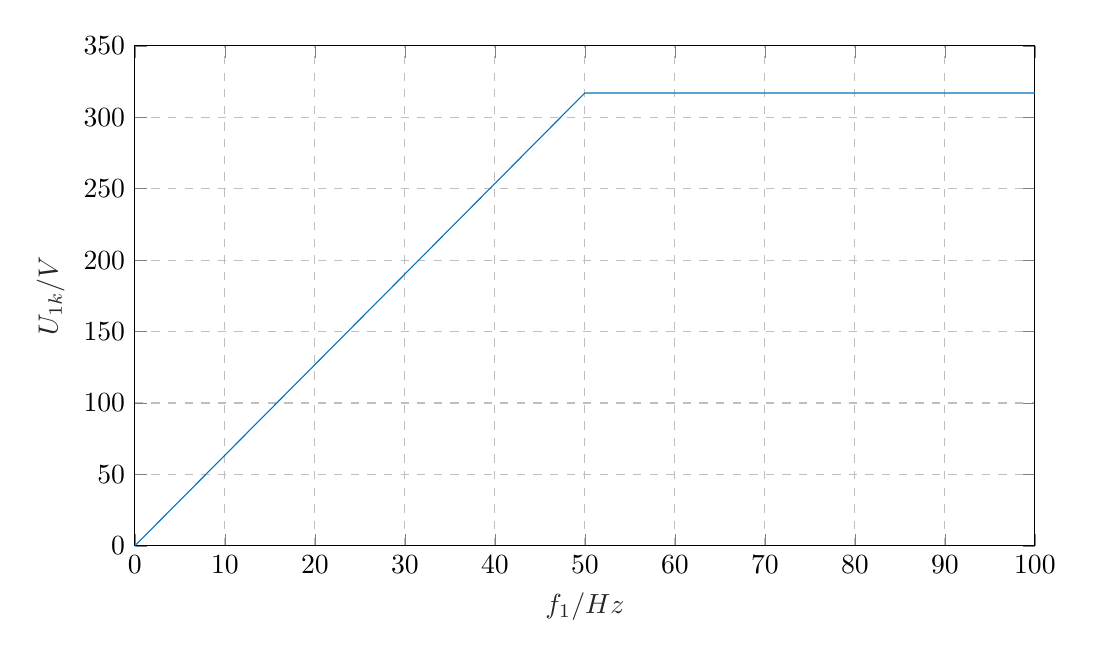
\begin{tikzpicture}

\begin{axis}[%
width=4.5in,
height=2.5in,
at={(0.758in,0.481in)},
scale only axis,
xmin=0,
xmax=100,
xtick={  0,  10,  20,  30,  40,  50,  60,  70,  80,  90, 100},
xlabel style={font=\color{white!15!black}},
xlabel={$ f_{1}/Hz $},
ymin=0,
ymax=350,
ytick={  0,  50, 100, 150, 200, 250, 300, 350},
ylabel style={font=\color{white!15!black}},
ylabel={$ U_{1k}/V $},
axis background/.style={fill=white},
xmajorgrids,
ymajorgrids,
major grid style={dashed}
]
\addplot [color=mycolor1, forget plot]
  table[row sep=crcr]{%
0	0\\
50	317\\
100	317\\
};
\end{axis}
\end{tikzpicture}%
	\caption{$ U/f_{1} $ - Kennlinie}
	\label{fig:3:UF}
\end{figure}

\section{}
Es soll nun ein Modell mit Simulink erstellt werden, welches ein Subsystem zeigt, mit dem die Darstellung der in Aufgabenteil a) entwickelten Funktionalität darstellen lässt.
\begin{itemize}
	\item Eingangsgröße System: Statorfrequenz; Ausgangsgröße System: Statorspannung
\end{itemize}
Es soll die Ausgangsspannung als Effektivwert der Außenleiterspannung zugegeben werden.

\begin{figure}[h]
	\centering
	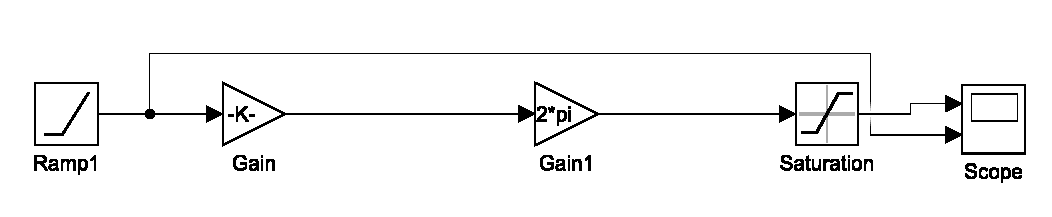
\includegraphics[width=0.7\textwidth]{./Bilder/Simulink-Modell.pdf}
	\caption{Simulink-Modell}
	\label{fig:3:simulink}
\end{figure}